\section{Results: soft wheat, 1959--2025}
\label{sec:wheat}

Wheat was the starting point of the project. Its results are null, but they are instructive: they show what the data can and cannot say, and they motivated the design of the maize analysis. I report them in two steps: the original analysis on 2010--2025, then the extension to 1959--2025.

\begin{figure}[H]
\centering
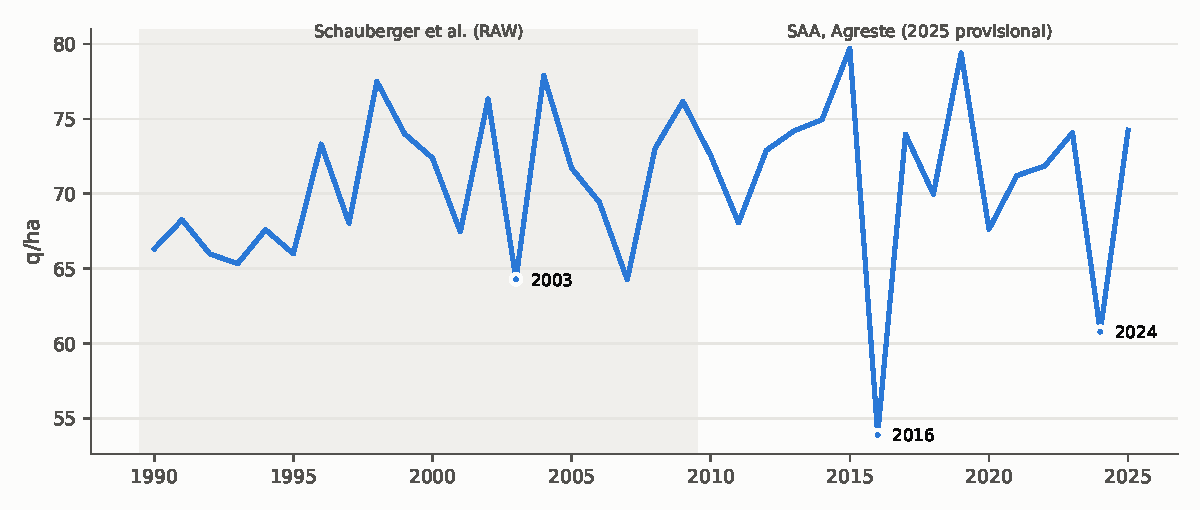
\includegraphics[width=0.95\textwidth]{figures/fig1_rendement_national.pdf}
\caption{Soft winter wheat yield, 1990--2025 (the full series starts in 1959), area-weighted mean of the 85 departments of the population. The shaded period comes from \textcite{schauberger2022}, the rest from the SAA. Yields have plateaued since the mid-1990s, a break also modelled by \textcite{gouache2015}; 2016 and 2024 are the two largest losses since 2010.}
\label{fig:wheat-yield}
\end{figure}

\subsection{2010--2025: a negative association that cannot be established}

\Cref{tab:wheat-short} reports the heat coefficient of the two pre-specified models, with the three inferences planned at the time.

\begin{table}[H]
\centering
\small
\caption{Wheat 2010--2025: heat above 32\,$^{\circ}$C in May--June}
\label{tab:wheat-short}
\begin{threeparttable}
{\setlength{\tabcolsep}{4pt}% GÉNÉRÉ par scripts/26_tables_memoire.py (phase4_principal.csv)
\begin{tabular}{lrrrrrrr}
\toprule
Model & $\hat\beta_2$ & \% per DD & \shortstack{$p$ clust.\\dept.} & \shortstack{$p$\\Conley} & \shortstack{$p$ boot.\\two-sided} & \shortstack{$p$ boot.\\one-sided} & $n$ \\
\midrule
M1 & $-0.0149$ & $-1.48$ & 0.004 & 0.047 & 0.374 & 0.189 & 1328 \\
M2 & $-0.0152$ & $-1.51$ & 0.007 & 0.111 & 0.327 & 0.164 & 1328 \\
\bottomrule
\end{tabular}
}
\begin{tablenotes}\footnotesize
\item M1: equation~\eqref{eq:m1}. M2: M1 plus the May--June soil wetness index and its square. 83 departments, 16 harvests. One-sided: in the direction of the hypothesis $\beta_2 < 0$.
\end{tablenotes}
\end{threeparttable}
\end{table}

Each degree-day above 32\,$^{\circ}$C during grain filling is associated with about \WheatPct\,\% lower yields. The sign is stable:
\begin{itemize}
  \item it is negative in \WheatRobPreNeg{} of the \WheatRobPreTot{} pre-specified robustness checks that change the coefficient (the exception extends the window to July), and in the \WheatRobAddTot{} checks added after the first estimates that estimate the same coefficient (R11--R13; R14 replaces it with temperature bins), defined before being computed;
  \item it is negative in all \LoyoTot{} estimates that leave out one year at a time;
  \item without the provisional year 2025, the association doubles, to about \WheatNoTwentyFivePct\,\% per degree-day.
\end{itemize}

Under the rule fixed in advance, which required all three inferences to agree, the association is not established. The bootstrap by year, the only test whose size was later found to be correct (\cref{sec:inference}), gives $p = \WheatPwcr$. Soil moisture tells the same story: the joint test of the two soil-moisture terms in M2 is highly significant with standard errors clustered by department ($p \WheatHtwoPdep$), and not with the bootstrap by year ($p = \WheatHtwoPwcr$).

This does not show that the effect is absent: the data carry little information on it. With 16 harvests and very hot early summers in only a few of them ($N_{\mathrm{eff}} = \NeffWheat$), a correctly sized test detects a true effect of $-1.5$\,\% only \WheatPowerWCR\,\% of the time (\cref{tab:power}).

\subsection{1959--2025: more years, still not enough}

The natural answer to too few years is more years. Over 1959--2025, the model M3 keeps the variables of M1 and adds department-by-period effects to absorb the breaks between data sources (\cref{sec:strategy}). \Cref{tab:wheat-long} reports the results.

\begin{table}[H]
\centering
\small
\caption{Wheat 1959--2025: heat above 32\,$^{\circ}$C in May--June (83 departments, \QtwoN{} observations)}
\label{tab:wheat-long}
% GÉNÉRÉ par scripts/26_tables_memoire.py (phase4bis_q2_hypotheses.csv, phase4bis_q2_robustesse.csv)
\begin{tabular}{lrrrr}
\toprule
& $\hat\beta_2$ & \% per DD & $p$ boot.\ two-sided & $p$ boot.\ one-sided \\
\midrule
\multicolumn{5}{l}{\emph{Heat slope, M3, and slopes by sub-period}} \\
All years, 1959--2025 (M3) & $-0.0108$ & $-1.08$ & 0.245 & 0.125 \\
Slope 1959--1981 & $-0.0014$ & $-0.14$ & 0.794 & 0.399 \\
Slope 1982--2003 & $-0.0279$ & $-2.75$ & 0.174 & 0.084 \\
Slope 2004--2025 & $-0.0113$ & $-1.13$ & 0.496 & 0.245 \\
\midrule
\multicolumn{5}{l}{\emph{Robustness of the main slope}} \\
Main (M3) & $-0.0108$ & $-1.08$ & --- & 0.125 \\
+ regional linear trends & $-0.0119$ & $-1.18$ & --- & 0.103 \\
Without 2025 (provisional) & $-0.0165$ & $-1.64$ & --- & 0.028 \\
1968--2025 (no missing yields) & $-0.0113$ & $-1.12$ & --- & 0.109 \\
Single department effect & $-0.0113$ & $-1.12$ & --- & 0.112 \\
Threshold 30\,$^{\circ}$C & $-0.0062$ & $-0.62$ & --- & 0.095 \\
\bottomrule
\end{tabular}

\end{table}

\paragraph{The main hypothesis is not established.} The association is \QtwoPct\,\% lower yield per degree-day, close to the estimate on 2010--2025, but a value this negative is not rare when there is no effect: the one-sided $p$-value is \QtwoP. The size of this test on these data is \QtwoSizeWCR\,\%, close to the nominal level in the placebo diagnostic. The sign is negative in all \QtwoRobTot{} robustness checks, and significant in \QtwoRobSig: the one without 2025 (one-sided $p = \QtwoNoTwentyFiveP$, two-sided $\QtwoNoTwentyFivePtwo$). I do not retain it. The rule was fixed in advance, and choosing the variant that ``works'' after seeing the results is exactly what pre-specification is meant to prevent. This sample also contains the 2010--2025 sample, so the similar estimate is not an independent replication.

\paragraph{Why more years did not help much.} Multiplying the number of harvests by four only raised the effective number of informative years from \NeffWheat{} to \NeffWheatLong. Before 2000, only one summer, 1976, brought substantial heat above 32\,$^{\circ}$C in May--June across the sample (\HeatSeventySix{} degree-days on average over the departments, against at most \HeatPreTwoThousandOtherMax{} in any other year before 2000), so most of the added years carry almost no information on it.

\paragraph{Has wheat become more or less sensitive?} The heat slope is $-\SlopeA$\,\% per degree-day over 1959--1981, $-\SlopeB$\,\% over 1982--2003 and $-\SlopeC$\,\% over 2004--2025. The joint bootstrap test that the three slopes are equal gives $p = \QtwoWaldP$; its size was not measured. I find no detectable change, but with so little information this is an absence of evidence, not evidence of stability. Varieties, sowing dates and practices also changed over these decades, so even a detected change would have been descriptive.

\subsection{What the wheat results teach}

Three lessons carried over to the maize analysis. A correct test can be a weak test, and it is better to know it before reading $p$-values. Adding years helps only if the added years contain the shock of interest. And a design that compares two outcomes exposed to the same summer, such as irrigated and rainfed maize in the same department, removes much of the common variation that makes the wheat estimates so imprecise.
